\documentclass{article}
\usepackage{apacite}
\usepackage{graphicx}
\usepackage{caption}
\usepackage{subcaption}
\graphicspath{ {./images/} }
\usepackage{amssymb}
\usepackage{mathtools}
\usepackage{multicol}
\title{\textbf{{\large LU3IN013}\\Research Project}\\{\Huge Formal Modeling of Algorithms\\for Distributed Systems}\\\textit{Final Report}}
\author{\Large\textbf{Tra My Nguyen}\\{\large 3702069}}
\date{\textit{2019-2020}}

\begin{document}
	
	\maketitle
	\pagenumbering{arabic}
	\newpage
	
	\section{Introduction}
	
	\subparagraph{}Distributed systems are omnipresent nowadays as they help resolving various computing problems with efficiency and high adaptability. However, along these advantages come a lot of difficulties due to the fact that entities in these systems run concurrently and can only communicate with each other via message-passing. As a result, coordinating the behavior of independent components of the system becomes the major challenge in distributed computing and one that is really hard to analyze. Instead of relying on traditional extensive testing, modern day system design uses formal methods based on mathematical techniques to study the reliability and robustness of a system. One proposal is the Carl Adam Petri's seminal work on Petri nets in the early 1960s.
	\subparagraph{}This project is carried out in responding to the Call for Models by the Model Checking Contest handled annually by LIP6, an event where formal verification tools for concurrent systems are evaluated in order to find the best suited techniques for a class of problem (e.g. state space generation, deadlock detection, reachability analysis, causal analysis). The goal is to create formal models with scaling capabilities from distributed algorithms using previously mentioned Petri nets, which may then be used alongside others in the contest as common benchmarks on which all tools will be compared.
	\subparagraph{}In this first report, I will be giving a general view on the notion of Petri nets and their functioning principle, as well as an initial application of Petri nets in modeling a Client-Server communication system. I will also be briefly presenting two distributed algorithms from which I will attempt to create Petri nets models and the steps I will take to work toward that goal.
	
	\section{Petri Net}
	\subparagraph{}Place/Transition Petri nets (P/T net) will be the main focus in this project.
			
	\begin{figure}[h]
		\centering
		\vspace*{-10pt}
		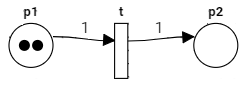
\includegraphics[scale=0.6]{net1}
		\caption{An simple P/T net}
		\vspace*{-10pt}
	\end{figure}
	\subparagraph{}
	The image above shows \textbf{a place/transition net (P/T net)}, which, at first glance, resembles a bipartite oriented weighted graph. Its vertices can be separated into a set of rectangle (known as transitions) and a set of circles (places), each circles containing a number of dots (tokens). A state of a P/T net is established by the number of tokens held by each place, formally defined by a marking. Transitions of a P/T net represent actions that can take place and modify its state. The cost of one action is indicated on its input arc (number of tokens taken away from the source place) and its product on the output arc (number of tokens added to the target place).
	\subparagraph{}The models to be produced in the project need to be scalable, which means by increasing a certain type of actors having similar behaviors in a system (parameters), we obtain multiple P/T nets describing the same scenario but of different sizes (number of transitions/places/arcs) or of different initial marking.
	\subsection{Formal definitions\cite{b1}}
	\subparagraph{}A P/T net can be hereby formally defined as\textit{ a tuple} $\mathcal{N} = (P,T,\textbf{Pre},\textbf{Post}),$ \textit{where
		\\$\bullet$ P is a finite set of \underline{places}, representing resources in a system, each place holds a number of \underline{tokens}, representing the number of occurrences of a resource
		\\$\bullet$ T is a finite set of \underline{transitions}, disjoint from P, representing actions that can occur in the system, and} 
		\\$\bullet$ \textbf{Pre},\textbf{Post} $\in\mathbb{N}^{|P|\times|T|}$ \textit{are matrices (the backward and forward incidence matrices of $\mathcal{N}$), \textbf{C} $=$ \textbf{Post} $-$ \textbf{Pre} is called the incidence matrix of $\mathcal{N}$.}
	\begin{table}[h]
		\begin{center}
			\begin{tabular}{ |c|c| } 
				\hline
				\textbf{Pre} & \textit{t}\\
				\hline
				$\textit{p}_{1}$ & 1\\ 
				$\textit{p}_{2}$ & 0\\ 
				\hline
			\end{tabular}
			%
			\begin{tabular}{ |c|c| } 
				\hline
				\textbf{Post} & \textit{t}\\
				\hline
				$\textit{p}_{1}$ & 0\\ 
				$\textit{p}_{2}$ & 1\\ 
				\hline
			\end{tabular}
			%
			\begin{tabular}{ |c|c| } 
				\hline
				\textbf{C} & \textit{t}\\
				\hline
				$\textit{p}_{1}$ & -1\\ 
				$\textit{p}_{2}$ & 1\\ 
				\hline
			\end{tabular}
			\caption{The incidence matrices of the P/T net in Figure 1}			
		\end{center}
	\end{table}
	\\A marking of a P/T net $\mathcal{N} = (P,T,\textbf{Pre},\textbf{Post})$ is a vector $\textbf{m}\in\mathbb{N}^{|P|}$. $\mathcal{N}$ \textit{together with a marking }$\textbf{m}_{0}$ \textit{(initial marking) is called} \textbf{a P/T net system} $\mathcal{S} = (\mathcal{N},\textbf{m}_{0})$. 
	\subparagraph{}It can be said that \textit{a transition $\mathit{t}\in\mathit{T}$ is enabled in a marking $\mathbf{m}$ if $\mathbf{m}\geq\mathbf{Pre}[\bullet,\mathit{t}]$. In this case } \textbf{the successor marking relation} \textit{is defined by $\mathbf{m}\xrightarrow{t}\textbf{m}'\Leftrightarrow \mathbf{m}\geq\mathbf{Pre}[\bullet,t]\land\mathbf{m}'=\mathbf{m}+\mathbf{Post}[\bullet,t]-\mathbf{Pre}[\bullet,t]=\mathbf{m}+\mathbf{C}[\bullet,t]$ ($\mathbf{Pre}[\bullet,t]$ denotes the t-column vector $ \mathbf{Pre}[\bullet,\mathit{t}]=(\mathbf{Pre}[p_{1},t],...,\mathbf{Pre}[p_{|P|},t])$) of the $|P|\times|T|$ matrix $\mathbf{Pre}$. The same holds for $\mathbf{Post}[\bullet,t]$ with respect to $\mathbf{Post}$.}
	\subparagraph{}Here, the initial marking is $\mathbf{m}_{0}=[2,0]>\mathbf{Pre}[\bullet,t]=[1,0]$, the transition \textit{t} is therefore fireable and firing it will lead to the successor marking $\mathbf{m}_{1}=[1,1]$.
	\begin{figure}[h]
		\centering
		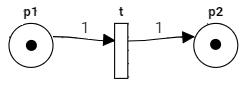
\includegraphics[scale=0.6]{net}
		\caption{New P/T net after firing transition $t$}
		\vspace*{-5pt}
	\end{figure}
	\section{The First Model: Client-Server System}
	\subparagraph{}Keeping in mind how a P/T net works, we can start modeling an P/T net simulating a simple communication channel between some clients and several servers. Each client can send a request to the channel, which will address it to one of the servers and transfer the reply back to the same client once the chosen server has responded.
	\begin{figure}[h]
		\centering
		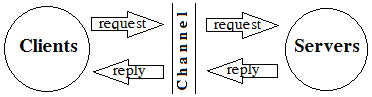
\includegraphics[scale=0.7]{cssys}
		\caption{Client-Server communication system}
	\end{figure}
	\subparagraph{}All models basically consist of 3 different parts: the clients, the servers and the channel connecting them. From now on, they will be highlighted respectively in orange, green and red. 
	\subparagraph{}Each actor has an initial stage represented by a place holding one token. A client$_i$ sending a request via the transition $\mathtt{send\_req_i}$ puts the channel to a new place $\mathtt{sys\_req_i}$ where it waits for an available server to help proceeding the request. After obtaining the reply, it enters the $\mathtt{sys\_rep_i}$ place, meaning it is ready to response to client$_i$ via transition $\mathtt{rec\_rep_i}$. Since the channel deals with one client at a time, there will be one set of these type of transitions and places for each client$_i$. Apart from the initial place, a server$_j$ is composed of as many $\mathtt{req_j\_c_i}$  transitions as there are clients because it can take a request from any client and only one at a time. 
	\begin{figure}[h]
		\centering
		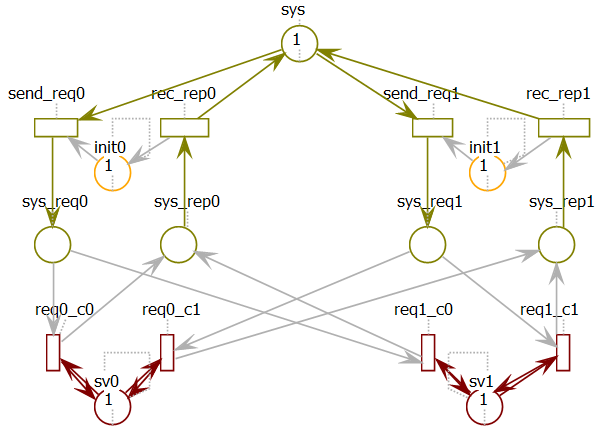
\includegraphics[scale=0.5]{cli2sv2_abs}
		\caption{Initial P/T net model of 2 clients and 2 servers}
	\end{figure}
	\subparagraph{}From this initial attempt, we can move on to expanding the client model by adding a $\mathtt{att_i}$ place where the client would wait for a reply.
	\begin{figure}[h]
		\centering
		\vspace*{10pt}
		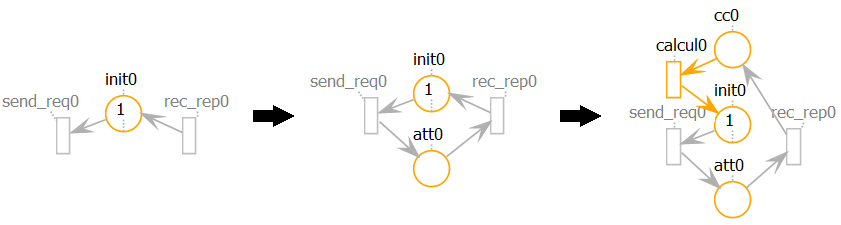
\includegraphics[scale=0.7]{client}
		\caption{Initial expansion of Client$_0$}
	\end{figure}
	\subparagraph{}For the server model, let's add a place named $\mathtt{sv_j\_c_i}$ between a server$_j$ receiving a request from the channel and giving a reply, where it would be handling the request of client$_i$. 
	\begin{figure}[h]
		\centering
		\hspace*{-50pt}
		\vspace*{10pt}
		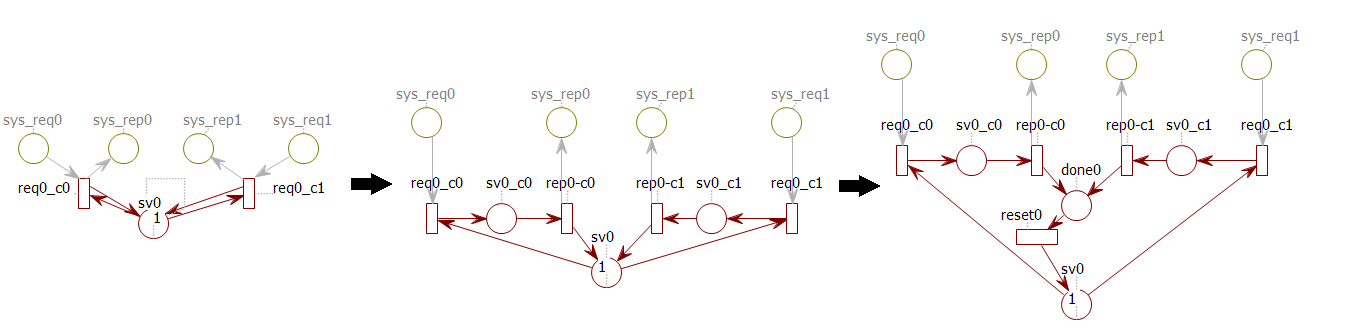
\includegraphics[scale=0.8]{server}
		\caption{Initial expansion of Server$_0$}
	\end{figure}
	\newpage
	\subparagraph{}The model now looks something like this.
	\begin{figure}[h]
		\centering
		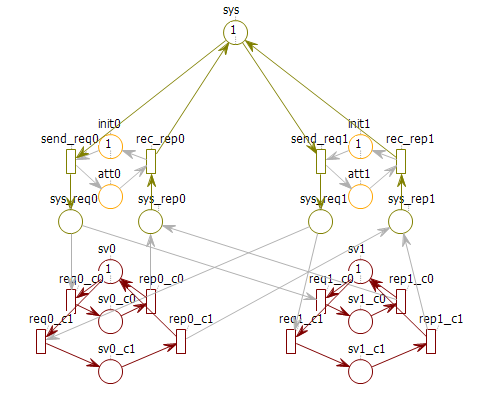
\includegraphics[scale=0.8]{cli2sv2_abs1}
		\caption{Expanded P/T net model of 2 clients and 2 servers}
	\end{figure}
	\subparagraph{}At the end, in order to increase the size of the net's state space, a possibility is to imagine the clients doing an extra step of calculation using their reply (place $\mathtt{cc_i}$ and transition $\mathtt{calcul_i}$) before returning to sending new requests and also, a resetting phase for the servers (place $\mathtt{done_j}$ and transition $\mathtt{reset_j}$).
	
	\begin{figure}[h]
		\centering
		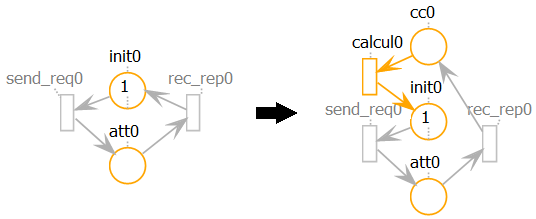
\includegraphics[scale=0.7]{client2}
		\caption{Second expansion of Client$_0$}
	\end{figure}

	\begin{figure}[h]
		\centering
		\hspace*{-60pt}
		\includegraphics[scale=0.75]{Server2}
		\caption{Second expansion of Server$_0$}
	\end{figure}
\newpage
	\subparagraph{}Here is the final model of 2 clients and 2 servers after combining the new client and server models with the initial channel model.
	\begin{center}
		\centering
		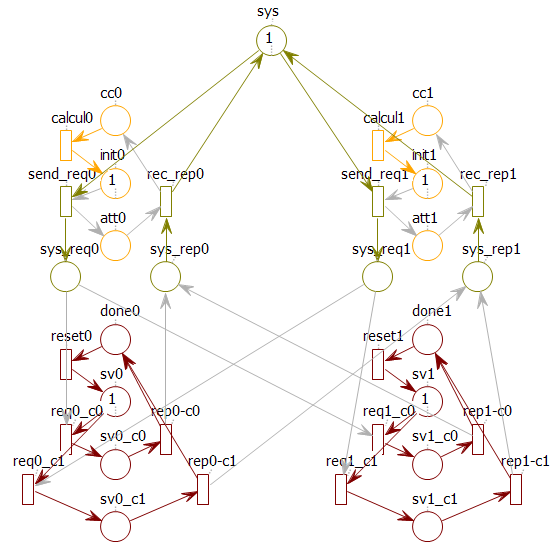
\includegraphics[scale=0.7]{cli2sv2}
		\vspace*{10pt}
		\\Figure 10: Final P/T net model of 2 clients and 2 servers
	\end{center}
	\subparagraph{}P/T nets of the same final type can be generated for a given number of clients and servers using a generator basing on the Java object-oriented language and the PNML Framework library. The idea of this generator follows simply each model of different actors explained above, each one implemented in its own class and finally, a common class Generator completes the net by connecting arcs between models (arcs in gray).
	\\Each model generated will possess these types of places and transitions:
		\\\textbf{Places}:
		\\\underline{Channel}
		\\$\bullet$ \texttt{sys}, waiting for request
		\\$\bullet$ \texttt{sys\_req$_{i}$}, having request from Client$_i$
		\\$\bullet$ \texttt{sys\_rep$_{i}$}, having reply for request of Client$_i$
		\\
		\underline{Client$_i$}
		\\$\bullet$ \texttt{init$_i$}, wanting to send request
		\\$\bullet$ \texttt{att$_i$}, waiting for reply
		\\$\bullet$ \texttt{cc$_i$}, ready to calculate
		\\
		\underline{Server$_i$}
		\\$\bullet$ \texttt{sv$_i$}, available
		\\$\bullet$ \texttt{sv$_i$\_c$_j$}, treating request from Client$_j$
		\\$\bullet$ \texttt{done$_i$}, done treating last request
		\\\\\textbf{Transitions}:
		\\\underline{Channel}
		\\$\bullet$ \texttt{send$_i$}, Client$_i$ sending request to channel
		\\$\bullet$ \texttt{receive$_i$}, Client$_i$ receiving reply from channel
		\\\underline{Client$_i$}
		\\$\bullet$ \texttt{calcul$_i$}, calculating
		\\\underline{Server$_i$}
		\\$\bullet$ \texttt{req$_i$\_c$_j$}, receiving request of Client$_j$ from channel
		\\$\bullet$ \texttt{rep$_i$\_c$_j$}, sending reply to request of Client$_j$ to channel
		\\$\bullet$ \texttt{reset$_i$}, resetting

	\section{Modeling distributed algorithms}
	\subsection{Leader election algorithm for bidirectional ring}
	\subsubsection{The algorithm \cite{b2}}
	\subparagraph{}Firstly, I will be looking at a classic problem in a distributed system: leader election, where node with the highest identity number in a network would be elected as the leader. The algorithm below, presented by D.S.Hirschberg and J.B.Sinclair(1980), shows the procedure of each node in a bidirectional ring network (where each node of identity $id_{i}$ has two neighbors $left_{i}$ and $right_{i}$ with whom it can communicate (send and receive messages)). 
	\begin{center}
		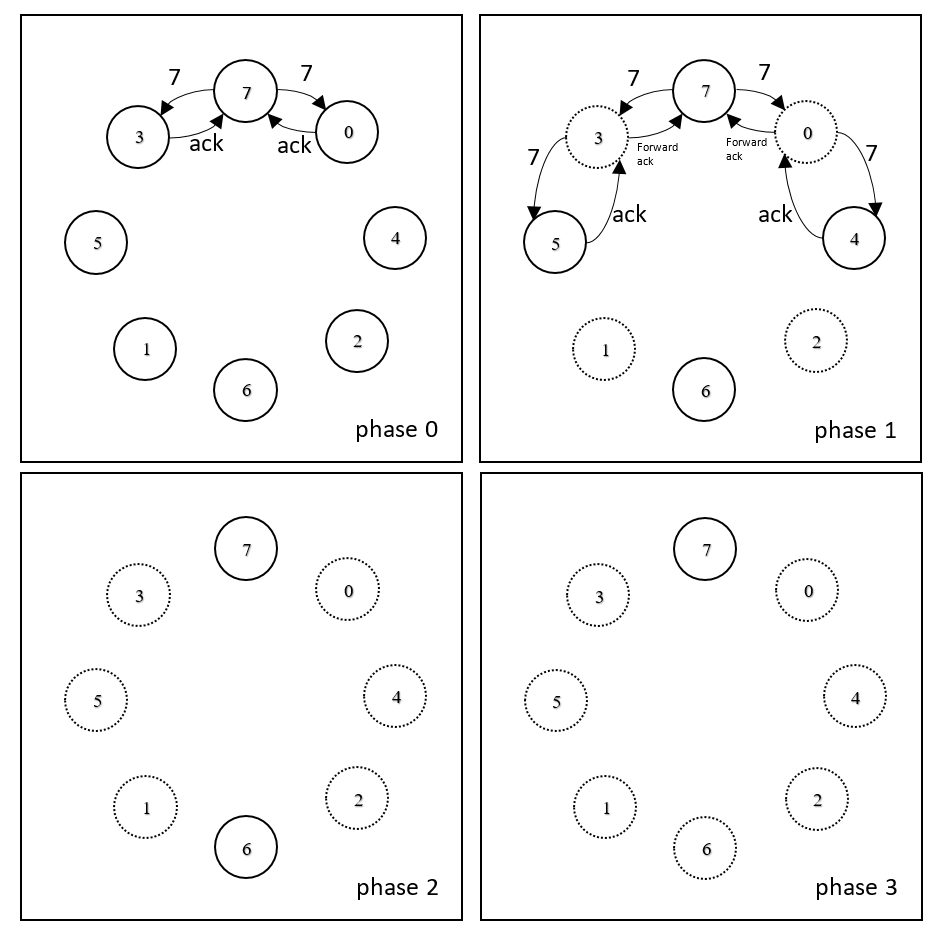
\includegraphics[scale=0.5]{Nlogn}
		\\Figure 11: Example of leader election in bidirectional 7-process ring network			
	\end{center}
	\subparagraph{}I will be modeling the behavior of each node, how they react to a message from another node. All nodes will receive a START message from exterior. Each node then sends ELECTION($id_{i},0,1$) to both of its neighbors, presenting its own identity, the first round number $r=0$ and the number of nodes its message has visited $d=1$. During each round \textit{r}, each node competes with its $2^{\mathit{r}}$ neighbors to the left and to the right, and only the winner of round \textit{r} can continue to round $\mathit{r}+1$. After one round, the identity of the winner of a neighborhood will be sent in a REPLY message back to the winner itself, a node receiving two REPLY messages from both sides learns that it is the winner of its $(2^{r}+1)$ neighborhood and moves on to the new round. The process ends with the node of highest identity number sending an ELECTION message to itself and becoming the leader, and then, all nodes learning the identity of the leader thanks to the ELECTED message.
	\begin{center}
		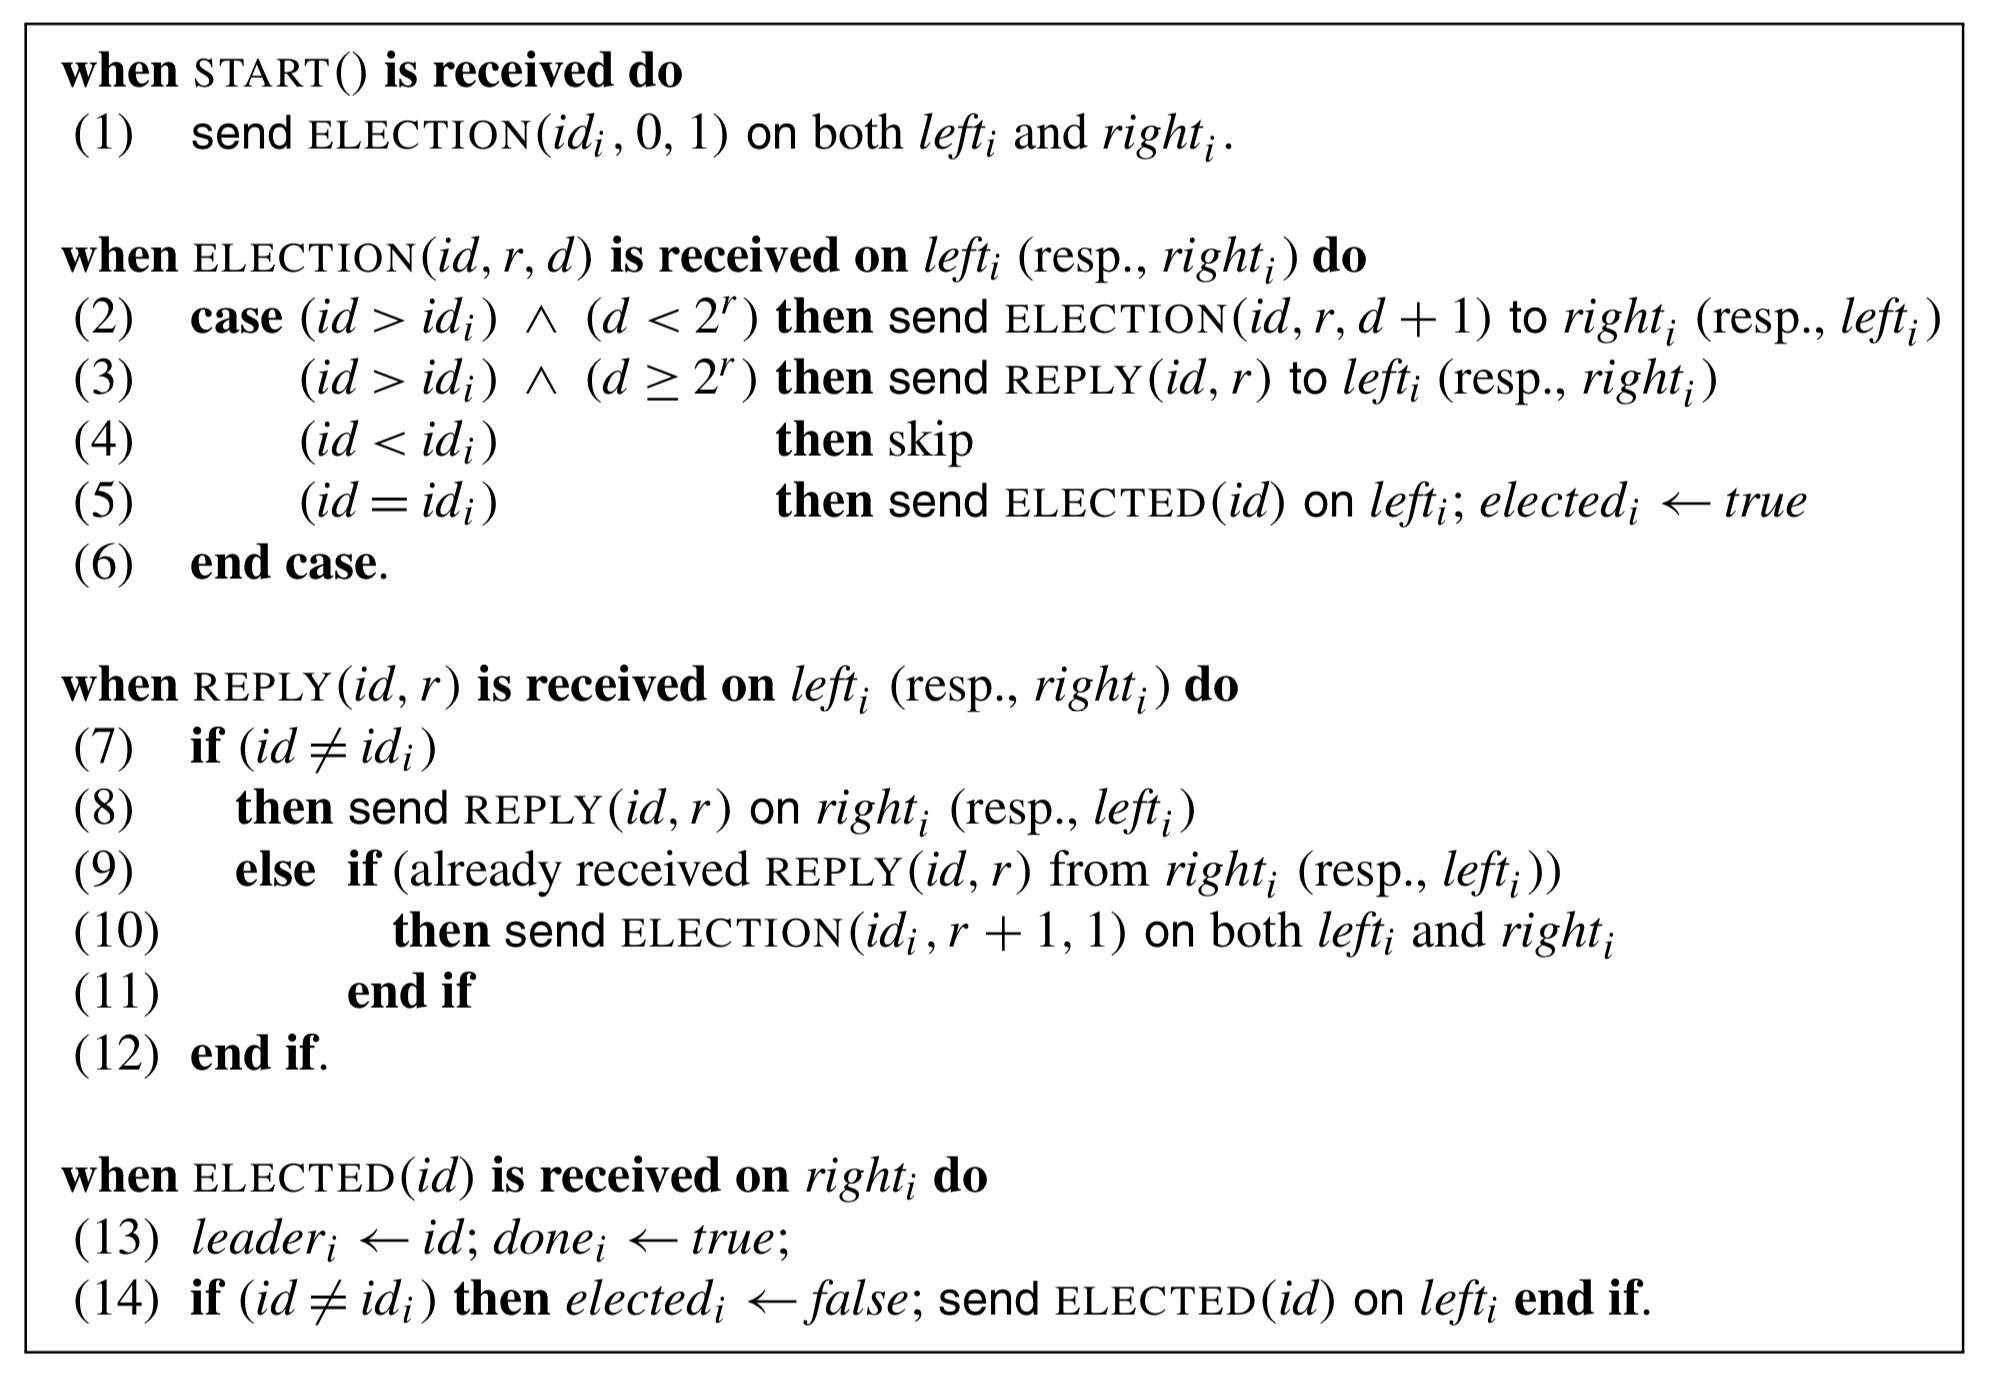
\includegraphics[scale=0.17]{IMG_7599}
		\\Figure 12: Leader election algorithm for bidirectional ring network		
	\end{center}
	\subsubsection{Modeling process}
	\subparagraph{}At the first look, the algorithm can be divided into two big parts: receiving START() and a loop for receiving other messages. 
	\subparagraph{}Upon receiving START() from exterior, a process$_i$ can send $ELECTION(id_i,0,1)$ to $left_i$ and $right_i$ (places  $\mathtt{election\_id\_0\_1\_to\_left}$ and  $\mathtt{election\_id\_0\_1\_to\_right}$) or it may enter the loop waiting for new messages (place $\mathtt{newmsg}$). Generally, there are 3 types of messages that can be sent to a process: ELECTION(), REPLY(), ELECTED(), all of which can be represented by transitions whose input places are $\mathtt{newmsg}$ of the receptor and, respectively, $\mathtt{election...}$, $\mathtt{reply...}$, $\mathtt{elected...}$ of the sender.
	\begin{center}
		\centering
		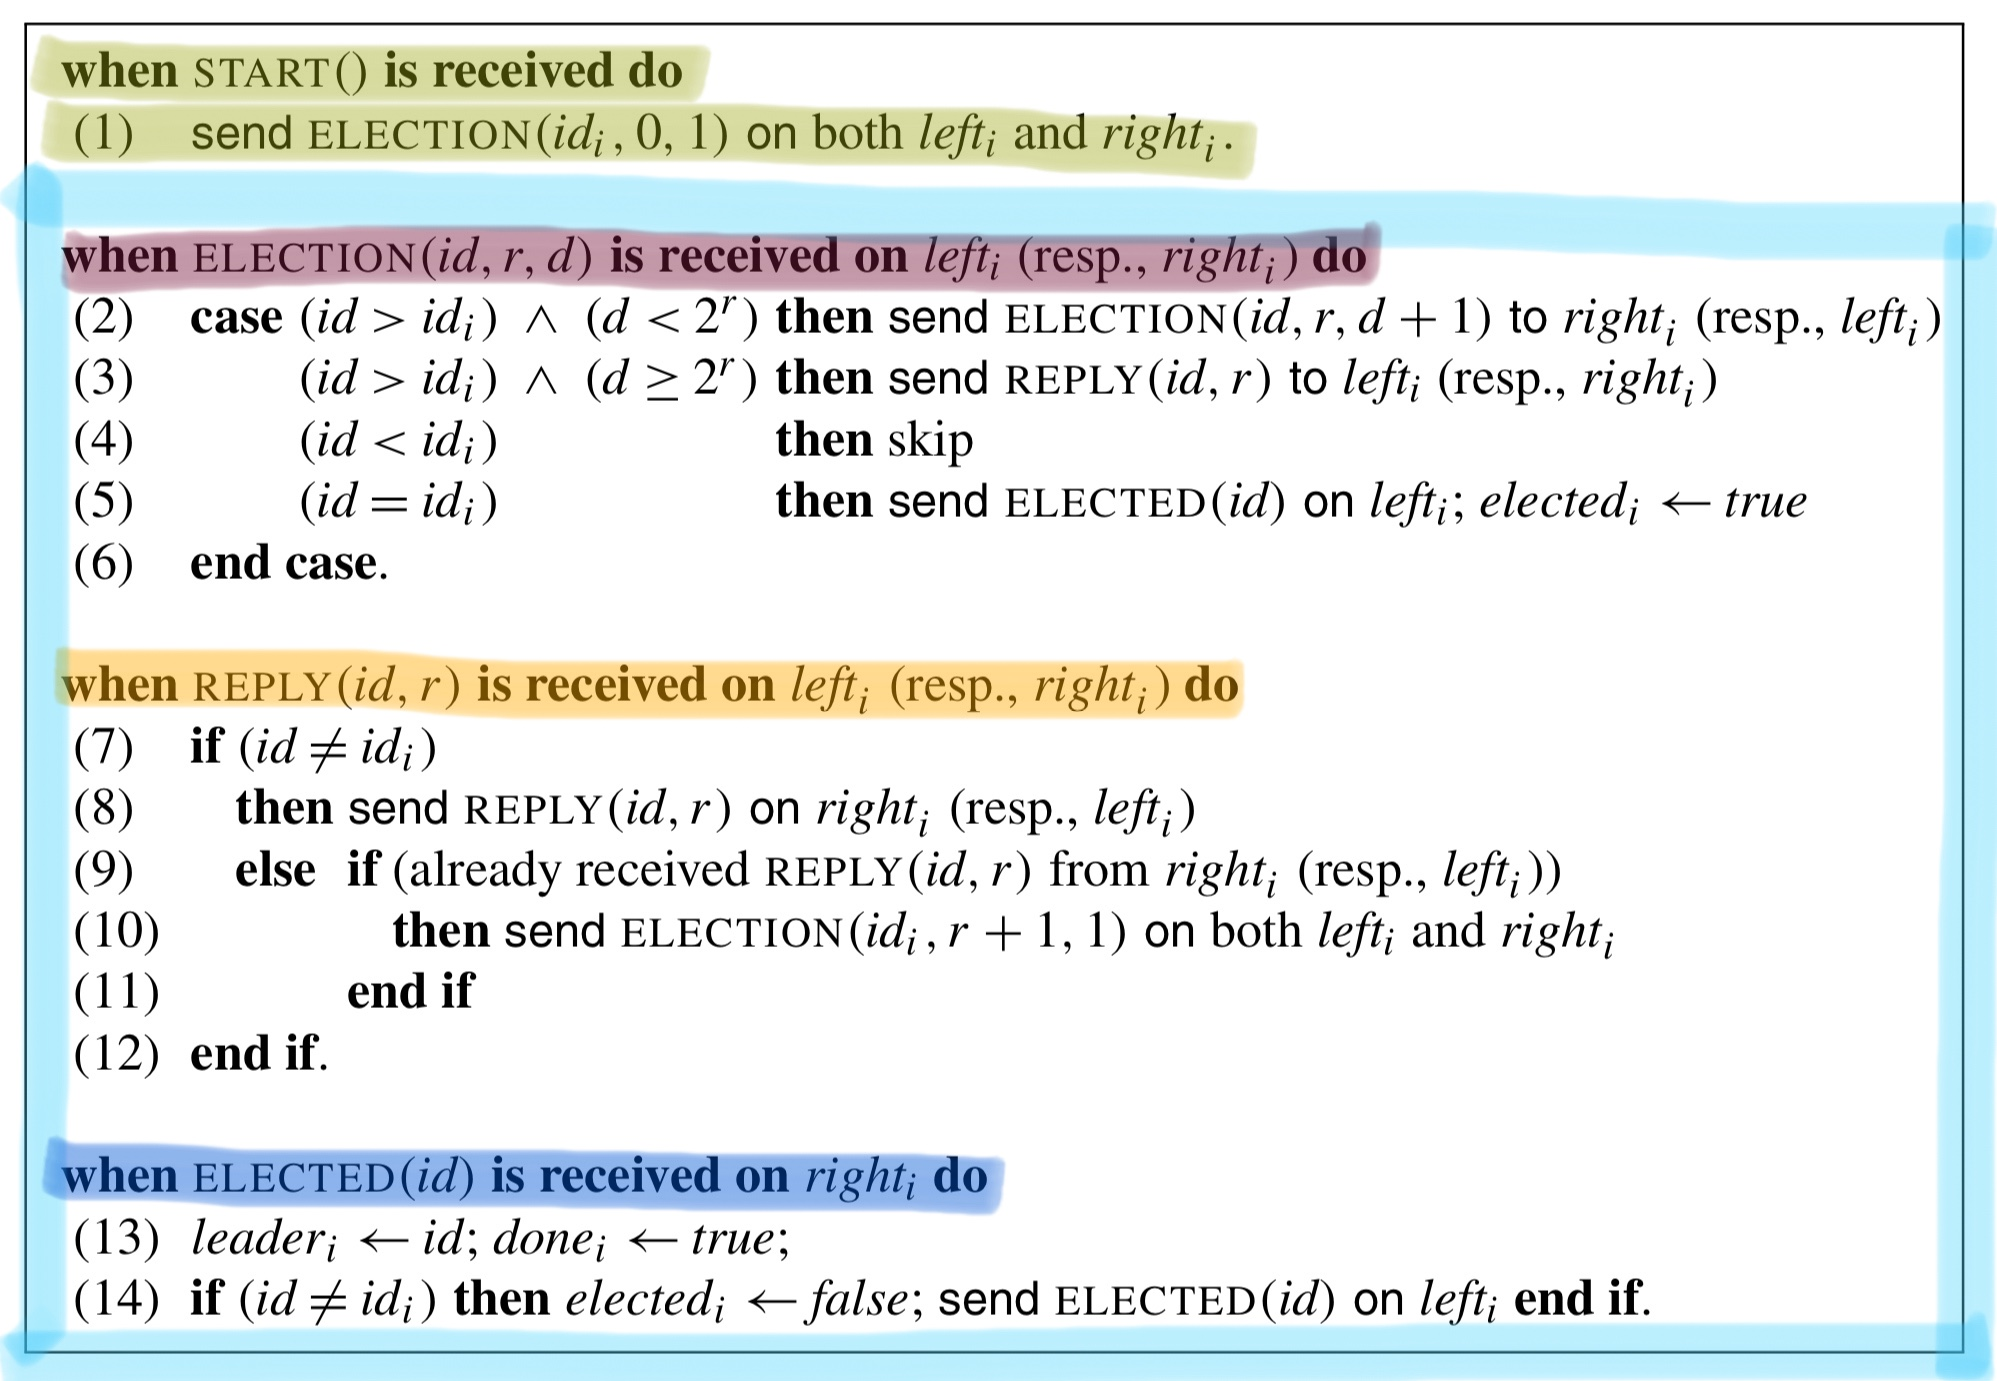
\includegraphics[scale=0.17]{IMG_7684}
		\vspace*{5pt}
		\\Figure 13: Initial take on the algorithm
	\end{center}
	\begin{center}
		\centering
		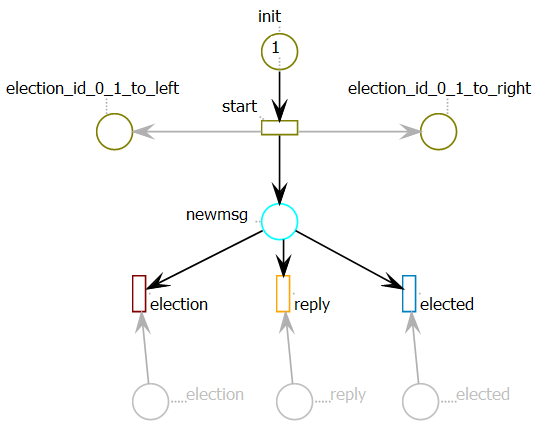
\includegraphics[scale=0.7]{process_init_2}
		\vspace*{5pt}
		\\Figure 14: Initial stage of a process
	\end{center}
	\subparagraph{}This initial part will be the same for every process.
	\newpage
	\subparagraph{}Next up, each message received can be broken down into small cases from which models can be built accordingly. Let's start with ELECTION() messages. In all cases, after dealing with the message, a process$_i$ needs to go back to the loop to continue receiving new messages (because $done_i \leftarrow true$ never happens). The $\mathtt{election}$ transition can result in a place (for preparing to send a message to another process (case a,b,d)) or nothing (for skipping this ELECTION() message (case c)).
	\begin{figure}[ht] 
		\begin{subfigure}[b]{0.5\linewidth}
			\centering
			\hspace*{-40pt}
			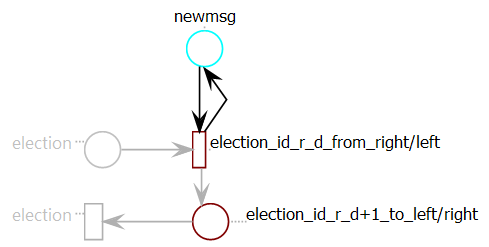
\includegraphics[scale=0.6]{election_cas1} 
			\caption{Case $(id>id_i) \wedge (d<2^r)$} 
			\label{fig13:a} 
			\vspace{4ex}
		\end{subfigure}%% 
		\begin{subfigure}[b]{0.5\linewidth}
			\centering
			\hspace*{20pt}
			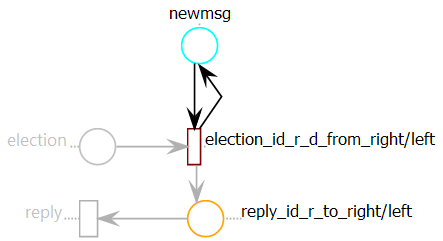
\includegraphics[scale=0.6]{election_cas2} 
			\caption{Case $(id>id_i) \wedge (d\geq2^r)$} 
			\label{fig13:b} 
			\vspace{4ex}
		\end{subfigure} 
		\begin{subfigure}[b]{0.5\linewidth}
			\centering
			\hspace*{-40pt}
			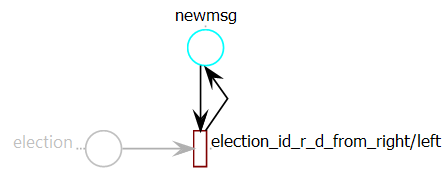
\includegraphics[scale=0.6]{election_cas3} 
			\caption{Case $(id<id_i)$} 
			\label{fig13:c} 
		\end{subfigure}%%
		\begin{subfigure}[b]{0.5\linewidth}
			\centering
			\hspace*{20pt}
			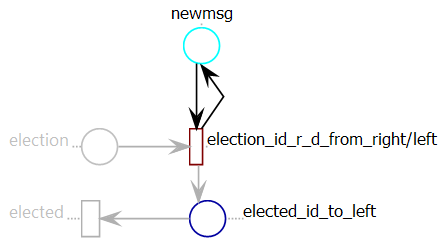
\includegraphics[scale=0.6]{election_cas4} 
			\caption{Case $(id=id_i)$} 
			\label{fig13:d} 
		\end{subfigure} 
		\\\begin{center}
			Figure 15: Models of different scenarios upon receiving ELECTION() message
		\end{center}
		\label{fig13} 
	\end{figure}

	\subparagraph{}Similarly to ELECTION() messages, a $\mathtt{reply}$ transition representing a REPLY() message needs to lead back to the $\mathtt{newmsg}$ place of the loop. There are 3 scenarios possible for the 2 conditions at line 7 and 9: \\- case a (true-NA), results in preparing to send a message to another process
	\\- case b (false-false), leads to a flag for keeping this REPLY() in memory
	\\- case c (false-true), results eventually in a transition $\mathtt{next\_round}$, meaning the process can move on to the next round and continue sending ELECTION() message carrying its own identity
	\newpage
	\begin{figure}[ht] 
		\begin{subfigure}[b]{0.5\linewidth}
			\centering
			\hspace*{-40pt}
			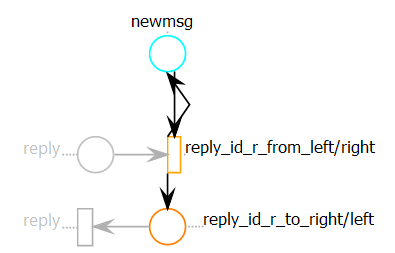
\includegraphics[scale=0.6]{reply_cas1} 
			\caption{Case $(id\neq id_i)$} 
			\label{fig14:a} 
			\vspace{4ex}
		\end{subfigure}%% 
		\begin{subfigure}[b]{0.4\linewidth}
			\centering
			\hspace*{10pt}
			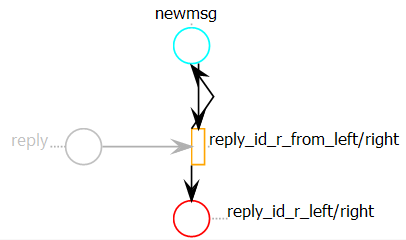
\includegraphics[scale=0.6]{reply_cas2} 
			\caption{Case $(id=id_i)$ and not yet received REPLY() from other side} 
			\label{fig14:b} 
			\vspace{4ex}
		\end{subfigure} 
		\begin{subfigure}[b]{1\linewidth}
			\centering
			\hspace*{30pt}
			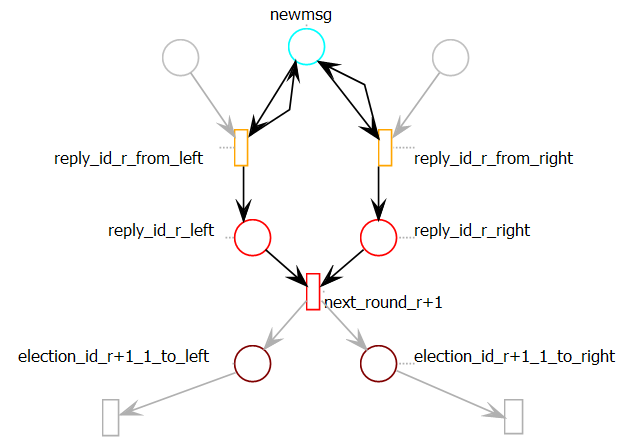
\includegraphics[scale=0.6]{reply_cas3} 
			\caption{Case$(id=id_i)$ and already received REPLY() from other side} 
			\label{fig14:c} 
		\end{subfigure}
		\\\begin{center}
			Figure 16: Models of different scenarios upon receiving REPLY() message
		\end{center}
		\label{fig14} 
	\end{figure}

	\subparagraph{}The last scenarios are when a process received ELECTED(), it then stops accepting new messages ($done \leftarrow true$) and for this reason, the transition $\mathtt{elected}$ does not go back to the $\mathtt{newmsg}$ loop. At this stage, the process will know whether it is elected, the transition leads then accordingly to the final place $\mathtt{elected}$ or $\mathtt{notelected}$. If a process is not elected, it will transfer the message to its left neighbor.
	\begin{figure}[ht] 
		\begin{subfigure}[b]{1\linewidth}
			\centering
			\hspace*{20pt}
			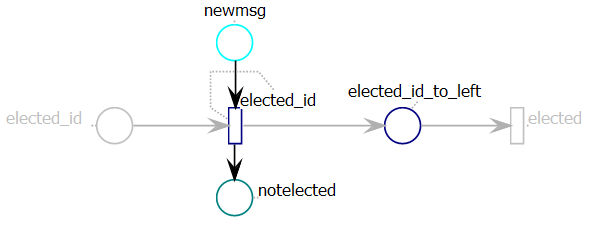
\includegraphics[scale=0.6]{elected_cas1} 
			\caption{Case $(id\neq id_i)$} 
			\label{fig15:a} 
		\end{subfigure}
		\begin{subfigure}[b]{1\linewidth}
			\vspace*{20pt}
			\centering
			\hspace*{-90pt}
			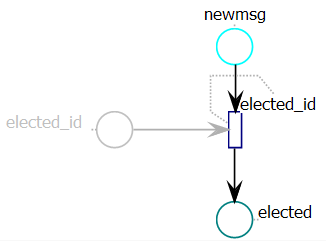
\includegraphics[scale=0.6]{elected_cas2} 
			\caption{Case $(id=id_i)$} 
			\label{fig15:b} 
		\end{subfigure} 
		\\\begin{center}
			Figure 17: Models of different scenarios upon receiving ELECTED() message
		\end{center}
		\label{fig15} 
	\end{figure}
\newpage
	\subparagraph{}Generally, for a ring of $n$ processes, $r\in \{0,...,\lceil log_2(n) \rceil \}$ and in each round r, $d\in \{1,...,2^r\}$. By the end of the operation,  $\mathtt{notelected}$ will hold $(n-1)$ tokens and $\mathtt{elected}$ only one. 
	\subparagraph{}The simplest scenario for a 2-process ring network can be obtained by enumerating all the message sent by each process and attaching each one to an above-mentioned scenario. In the model below, process$_1$ to the left and process$_2$ to the right both go from their initial stage through 2 rounds of communication to learn their final status at the last stage. However, the messages they receive vary according to their identity.
	\begin{center}
		\vspace*{-50pt}
		\hspace*{-100pt}
		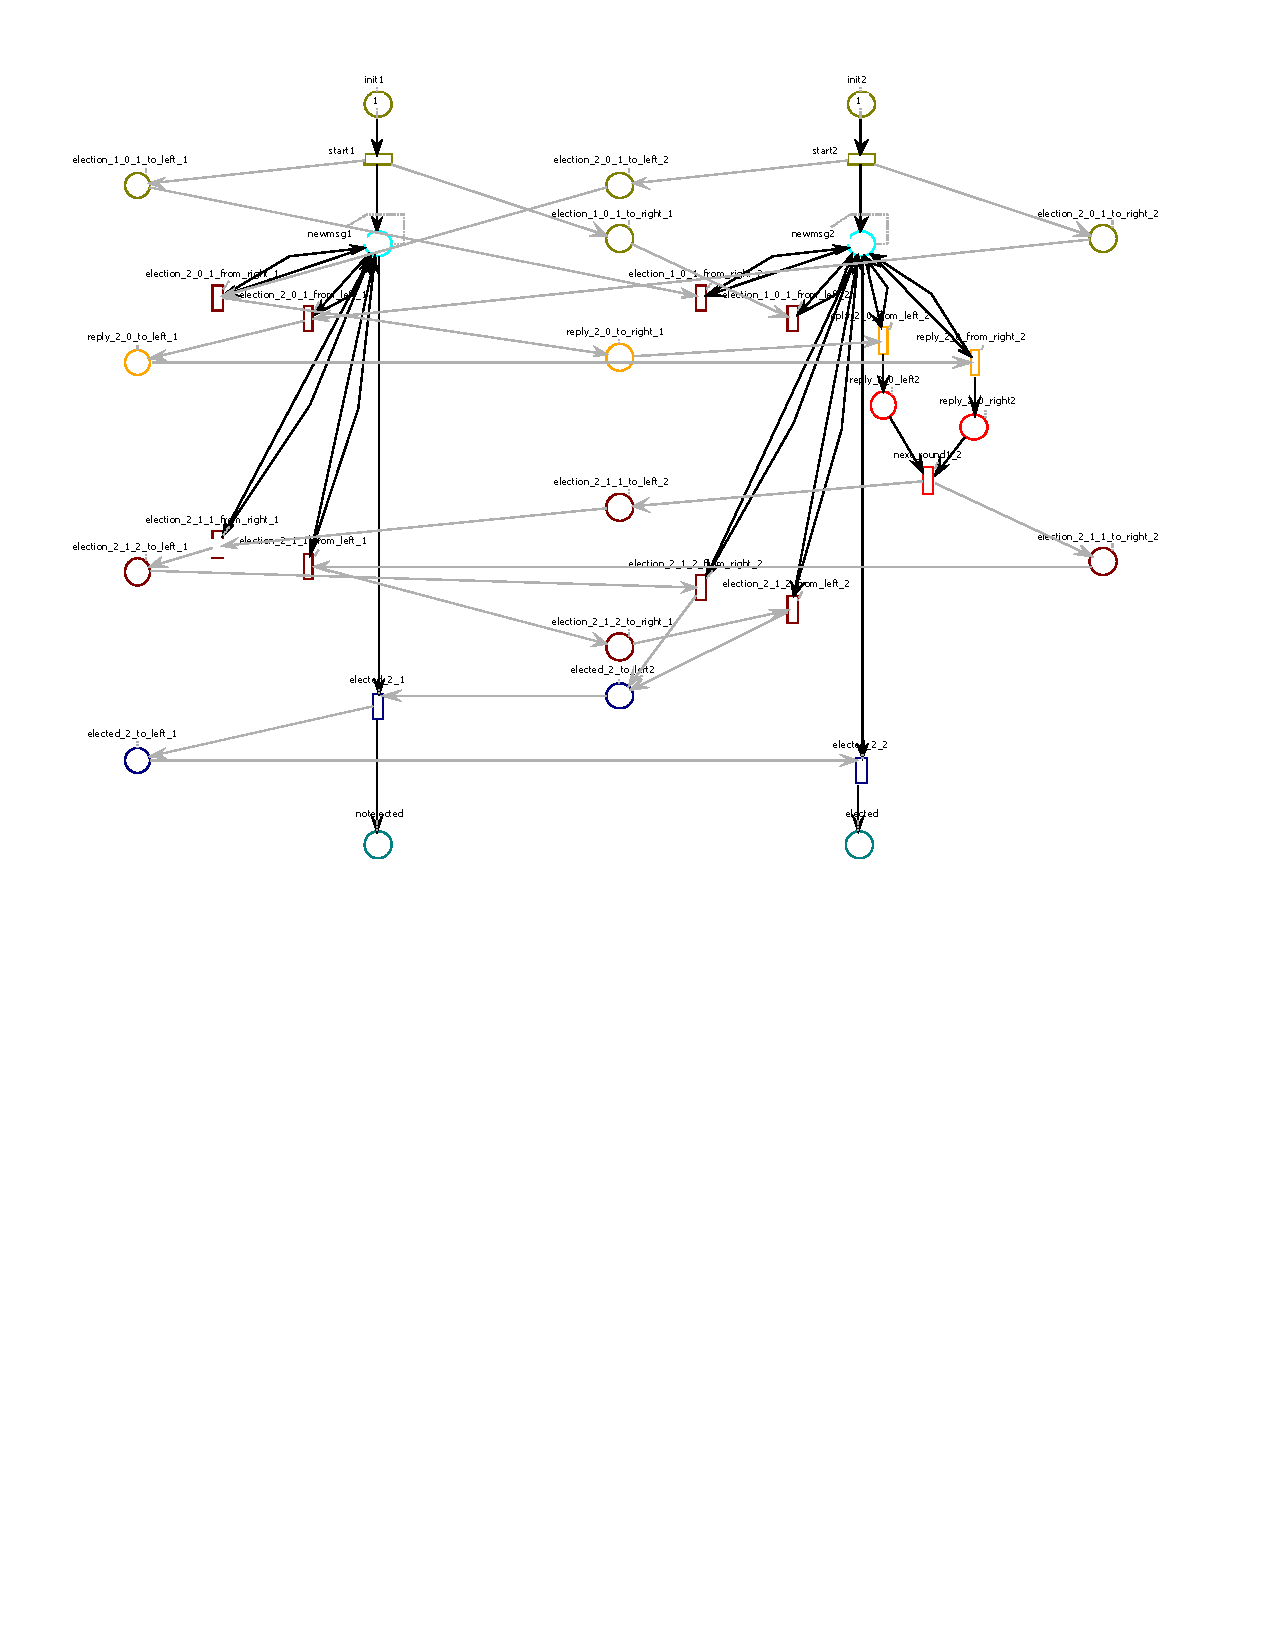
\includegraphics[scale=0.9,trim=0 370 0 30,clip]{ring2_abs}
		\\Figure 18: P/T net model of leader election on\\ bidirectional 2-process ring network
	\end{center}
	\subparagraph{}Lastly, we can go further by expanding all $\mathtt{election}$ and $\mathtt{reply}$ transitions.
	\begin{center}
		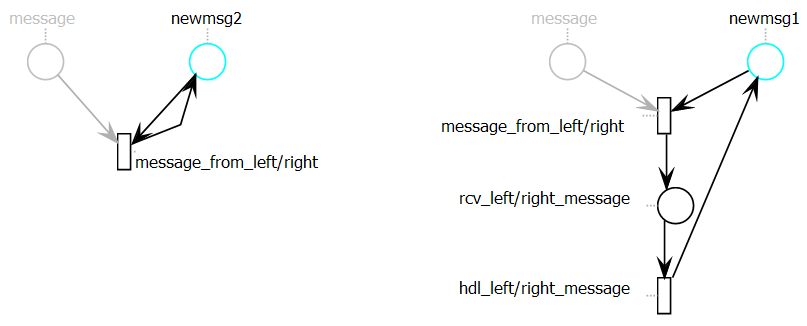
\includegraphics[scale=0.5]{ring_expanded}
		\\Figure 19: Expansion of $\mathtt{election}$ and $\mathtt{reply}$ transitions
	\end{center}
	\begin{center}
		\hspace*{-120pt}
		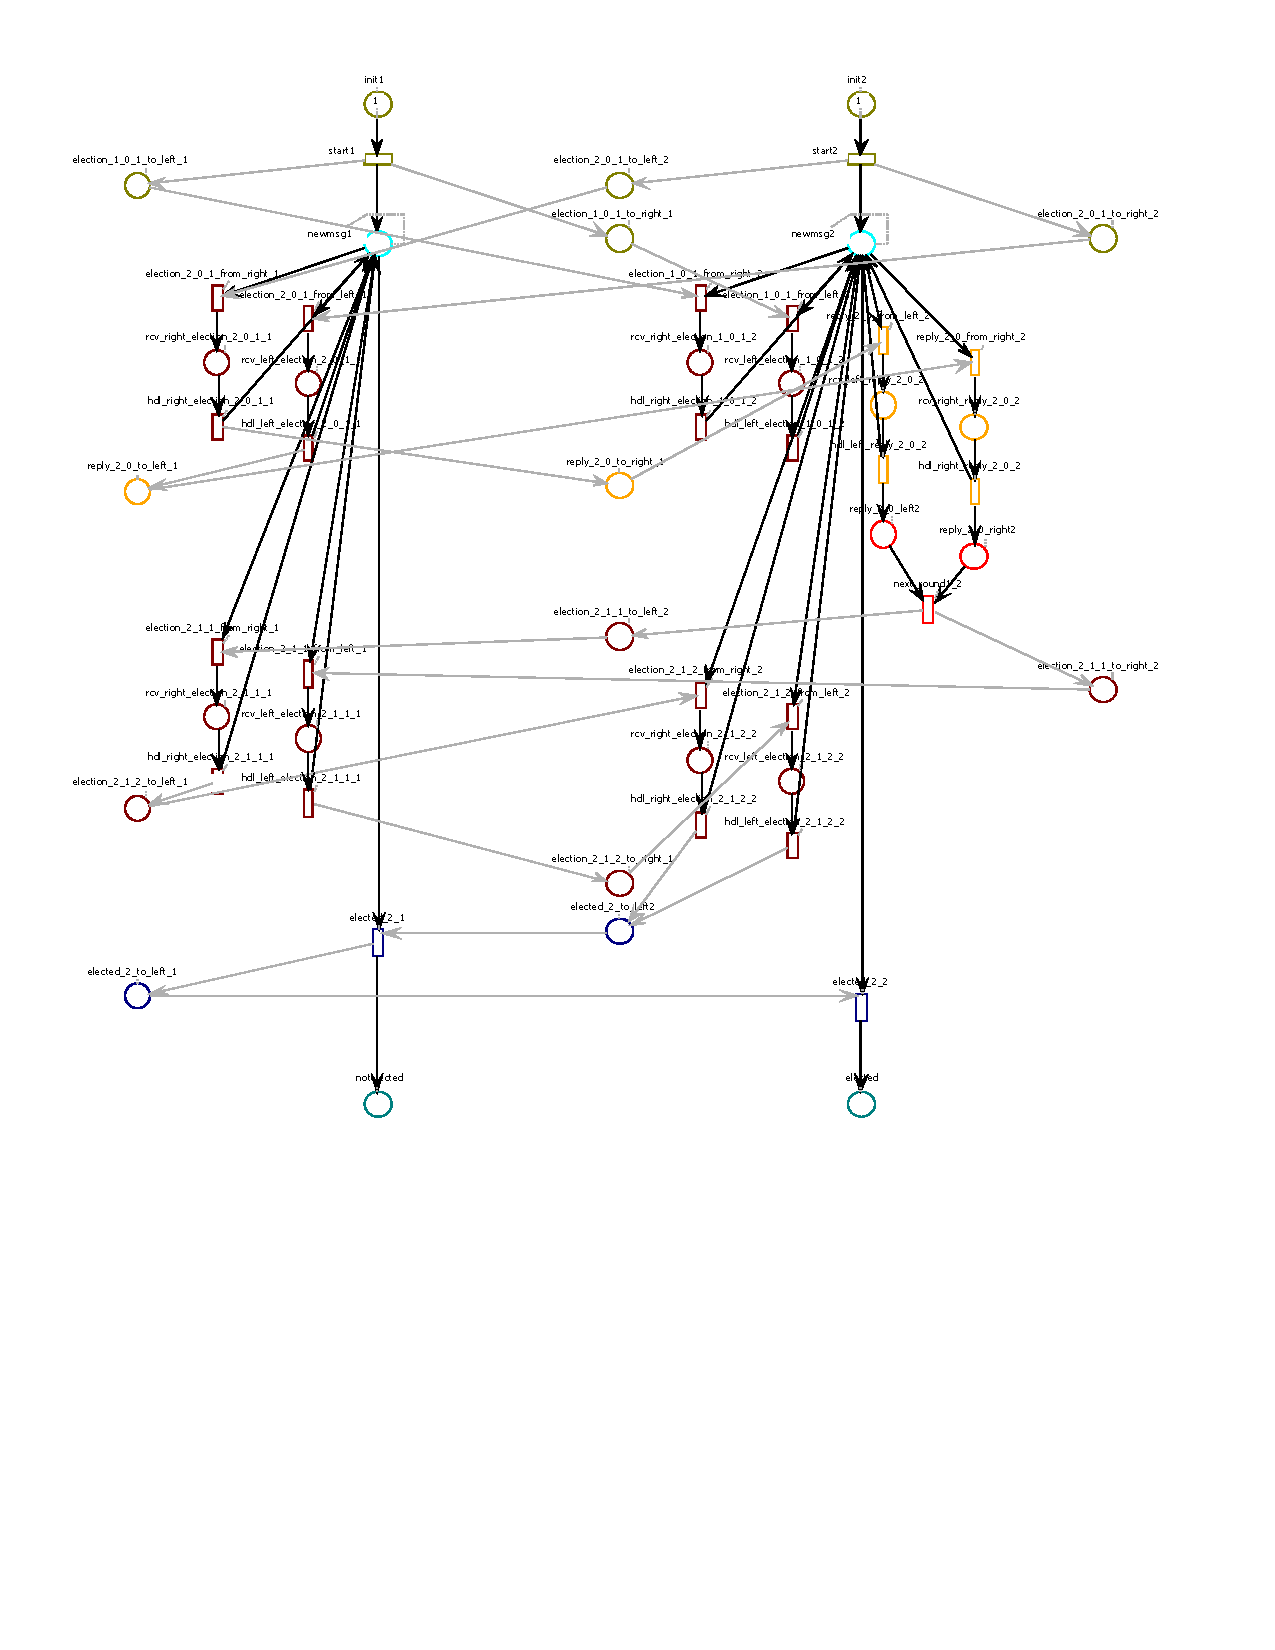
\includegraphics[scale=1,trim=0 250 0 35,clip]{ring2}
		\\Figure 20: Final P/T net model of leader election on\\ bidirectional 2-process ring network
	\end{center}
	\subparagraph{}The generator for this type of model uses the same principle of enumerating messages and attaching small models onto the whole ring. After generating the initial stage for all processes, it will list, for each round $r$, all the possible consequences of the ELECTION() messages sent by a competitor process$_i$ to its neighborhood and then, connect all the fitting models with each others and onto the main ring (arcs in gray). The chosen ring configuration for this project is an increasing one ($... \leftrightarrow 1 \leftrightarrow 2 \leftrightarrow 3 \leftrightarrow ...$), though, the generator can be modified very easily to fit other configurations.
	\\The result will consist of these types of place and transition:
	\\\textbf{\underline{Places}}
	\\$\bullet$ \texttt{init$_{i}$}, initial state of process $p_i$
	\\$\bullet$ \texttt{newmsg$_{i}$}, $p_i$ available to receive messages
	\\$\bullet$ \texttt{election\_id\_r\_d/reply\_id\_r\_to\_right/left\_i}, $p_i$ ready to send ELECTION(id,r,d)/ REPLY(id,r) to $right_i$/$left_i$
	\\$\bullet$ \texttt{rcv\_right/left\_election\_id\_r\_d/reply\_id\_r\_i}, $p_i$ just received ELECTION(id,r,d)/ REPLY(id,r) from $right_i$/$left_i$
	\\$\bullet$ \texttt{reply\_i\_r\_right/left\_i}, $p_i$ has already received REPLY(i,r) from $right_i$/$left_i$	
	\\$\bullet$ \texttt{elected\_id\_to\_left\_i}, $p_i$ ready to send ELECTED(id) to its $left_i$
	\\$\bullet$ \texttt{elected}, elected leader
	\\$\bullet$ \texttt{not\_elected}, not elected processes
	\\\\\textbf{\underline{Transitions}}
	\\$\bullet$ \texttt{start$_{i}$}, $p_i$ receiving START() from exterior
	\\$\bullet$ \texttt{election\_id\_r\_d/reply\_id\_r\_from\_right/left\_i}, $p_i$ receiving ELECTION(id,r,d)/ REPLY(id,r) from $right_i$/$left_i$
	\\$\bullet$ \texttt{hdl\_right/left\_election\_id\_r\_d/reply\_id\_r\_i}, $p_i$ handling ELECTION(id,r,d)/ REPLY(id,r) sent by $right_i$/$left_i$
	\\$\bullet$ \texttt{next\_round$_{r}\_i$}, $p_i$ moving to round $r$
	\\$\bullet$ \texttt{elected\_id\_i}, $p_i$ receiving elected(id) from $right_i$
	\subsection{Bellman-Ford's shortest path algorithm}
	\subsubsection{The algorithm \cite{b2}}
	\subparagraph{}Secondly, I will turn to an algorithm that I have studied in the sequential context: Bellman-Ford's Shortest Path Algorithm, and try to model its distributed adaptation. The goal is that each vertex in a non-oriented weighted graph learns the shortest path from itself to every other vertex. It is based on the principle of dynamic programming where each vertex $p_{j}$ stores an array $length_{i}[1..n]$ such that $length_{i}[k]$ will contain the length of the shortest path from $p_{i}$ to $p_{k}$ (initially, $length_{i}[i]=0$ and $length_{i}[k]=+\infty$ for $k \neq i$). When a node $p_{i}$ updates its $length_{i}$ (by comparing the length of the newly learned and the old path and updating if the new path is shorter), it will signal all of its neighbors $p_{j}$ to update their own $length_{j}$ array. For a node $p_{i}$, $l_{g_{i}}[j]$ denotes the length associated with the channel $(i,j)$ and $routing\_to_{i}[1...n]$ is such that $routing\_to_{i}[k]=j$ means that $p_{j}$ is a neighbor of $p_{i}$ on a shortest path to $p_{k}$. The algorithm ends when each node acquires the knowledge of the shortest path to other nodes, there will not be anymore UPDATE message as the condition in which $update_{i}$ becomes $true$ can no longer be satisfied.
	\begin{center}
		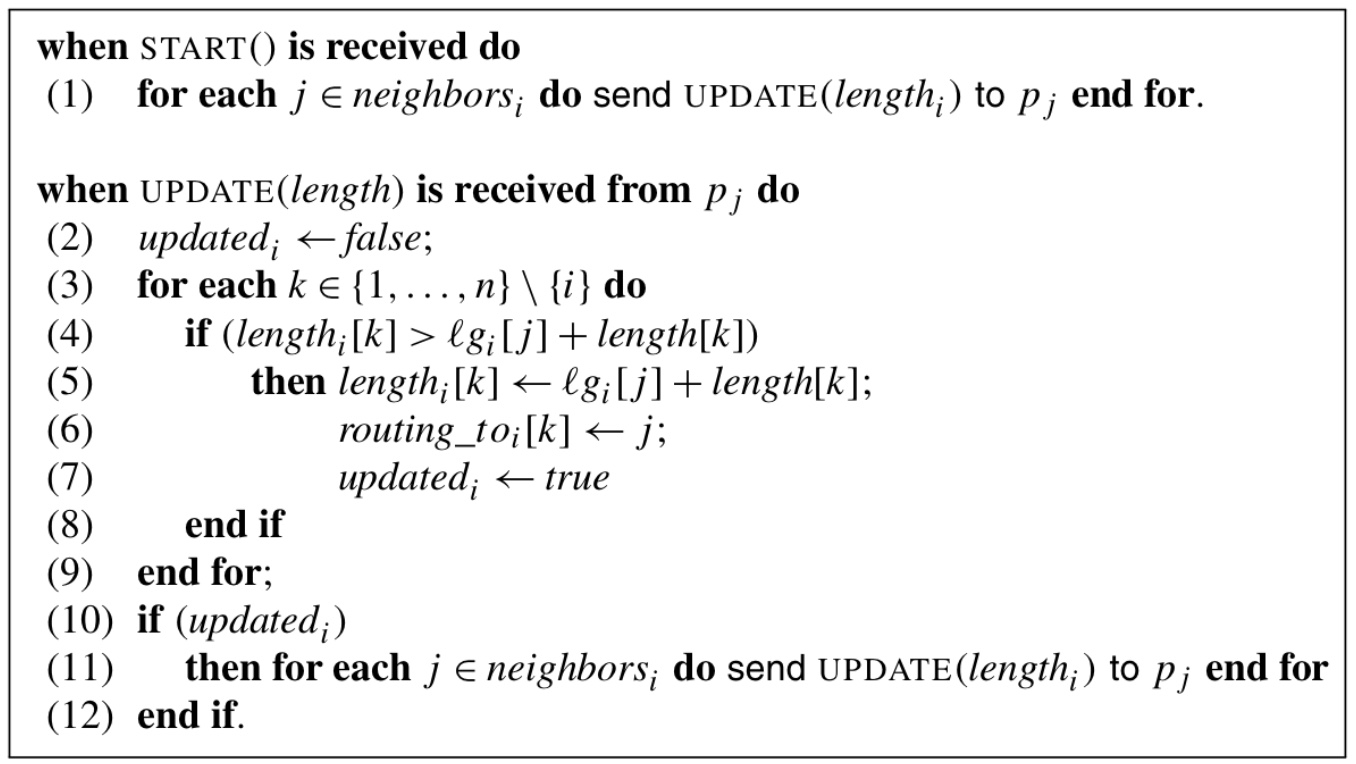
\includegraphics[scale=0.25]{IMG_7653}
		\\Figure 5: Distributed adaptation of Bellman-Ford's Shortest Path algorithm
	\end{center}
	\subsubsection{Modeling process}
	\subparagraph{}Unfortunately, the modeling of this algorithm could not be done in time. An naive start would be something resembling the model of leader election, an similar initial stage with a loop for receiving new messages.
	\section{Conclusion}
	\subparagraph{}Through this project, I have learned the concept of Petri nets some of its simple applications, which helped me gain a better understanding of the field of concurrent programming. The work of modeling has taught me to capture the essentials of algorithms, and from that, I was able to visualize and look at them in a new way. Even though, due to lack of time, I could only create two simple models, I hope they are interesting enough and will be of use for the MCC.
\bibliographystyle{apacite}
\bibliography{bibpjrech}
\end{document}